\subsection{Simulações Numéricas}

Consideramos 4 configurações de poço para as simulações: $A_1$ (anular concêntrico sem erosões); $A_2$ (anular excêntrico sem erosões); $B_1$ (anular concêntrico com erosões); $A_2$ (anular excêntrico com erosões). Para calcular o coeficiente de eficiência de varrido do colchão lavador, escolhemos 4 cotas de profundidade, a saber $y_k = \{0,1; 0,3; 0,7; 1.0\}$, assim retornando os respectivos valores $\eta(y_k)$, para $k=1,2,3,4$ para as porções esquerda e direita do anular. O \textit{loop} temporal considerou um passo de tempo $\Delta t = 0.00025$ com 40 mil iterações. Cada simulação durou, em média, 3 horas, em um computador com processador Intel Core i5 8a. geração e 8 GB RAM.

\subsubsection{Configurações sem Erosões}

Considerando a geometria sem nenhum tipo de erosão na parede do poço e com valor de \textit{standoff} 100\% $A_1$, é possível observar na Fig. \ref{fig:perfil_velocidade_liso_saida_paraview_10s} o efeito de escoamento parabólico na saída do espaço anular.
\begin{figure}[H]
        \centering
    	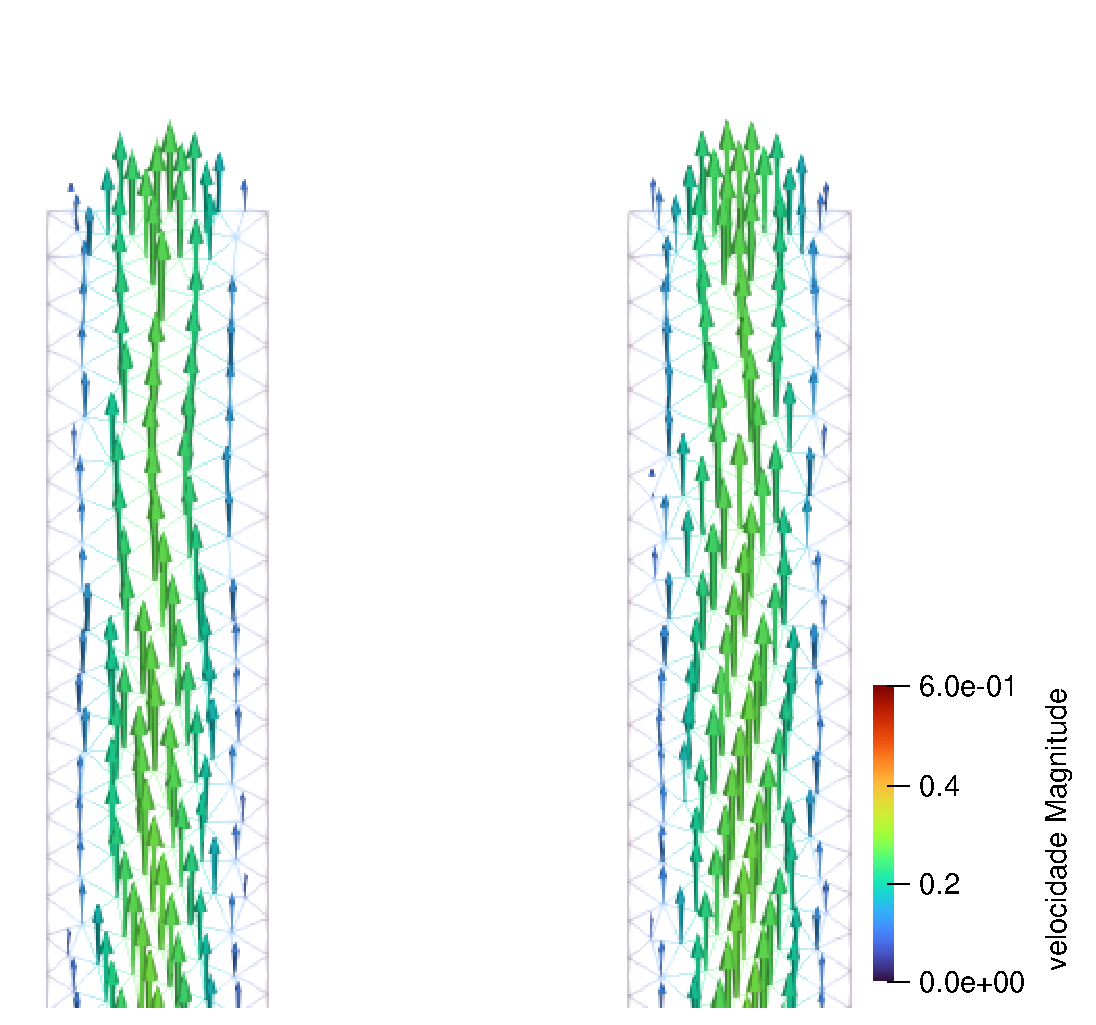
\includegraphics[scale=0.5]{img/perfil_vel/liso/perfil_de_vel_saida_paraview.eps}
    	\caption[Campo de velocidade na saída do espaço anular no tempo de 10s na geometria $A_1$.]{Campo de velocidade na saída do espaço anular no tempo de 10s na geometria $A_1$. Fonte: autor}
    	\label{fig:perfil_velocidade_liso_saida_paraview_10s}
\end{figure}
    
A Fig. \ref{fig:perfil_velocidade_liso_sapata_paraview_0_5s} é o perfil de velocidade no tempo de 0,5 segundo. Podemos observar a simetria do escoamento por se tratar de um caso com excentricidade nula. 
\begin{figure}[H]
        \centering
        \begin{subfigure}[b]{0.42\linewidth}
    		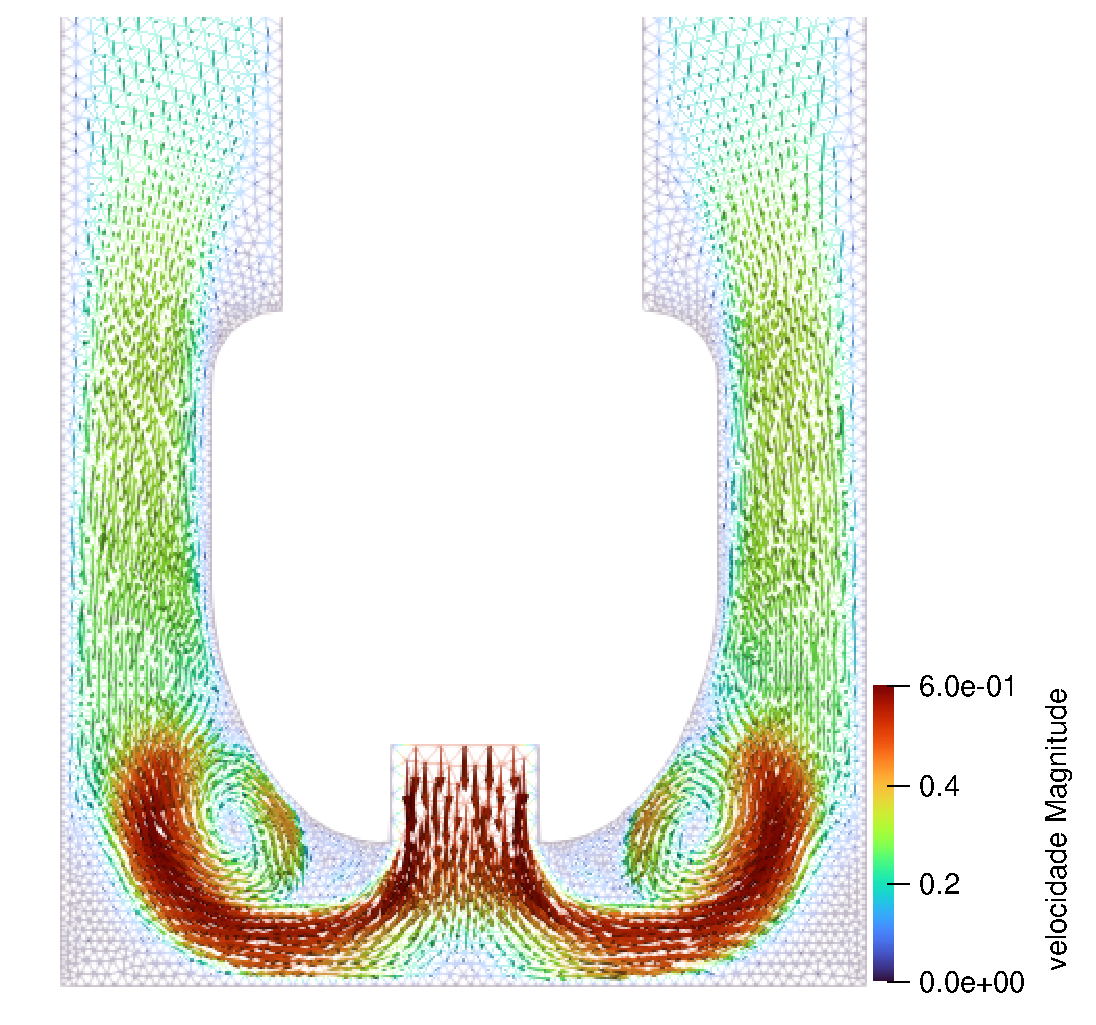
\includegraphics[width=\linewidth]{img/perfil_vel/liso/perfil_de_vel_sapata_paraview_0.5s.eps}
    	\end{subfigure}
    	\begin{subfigure}[b]{0.42\linewidth}
    		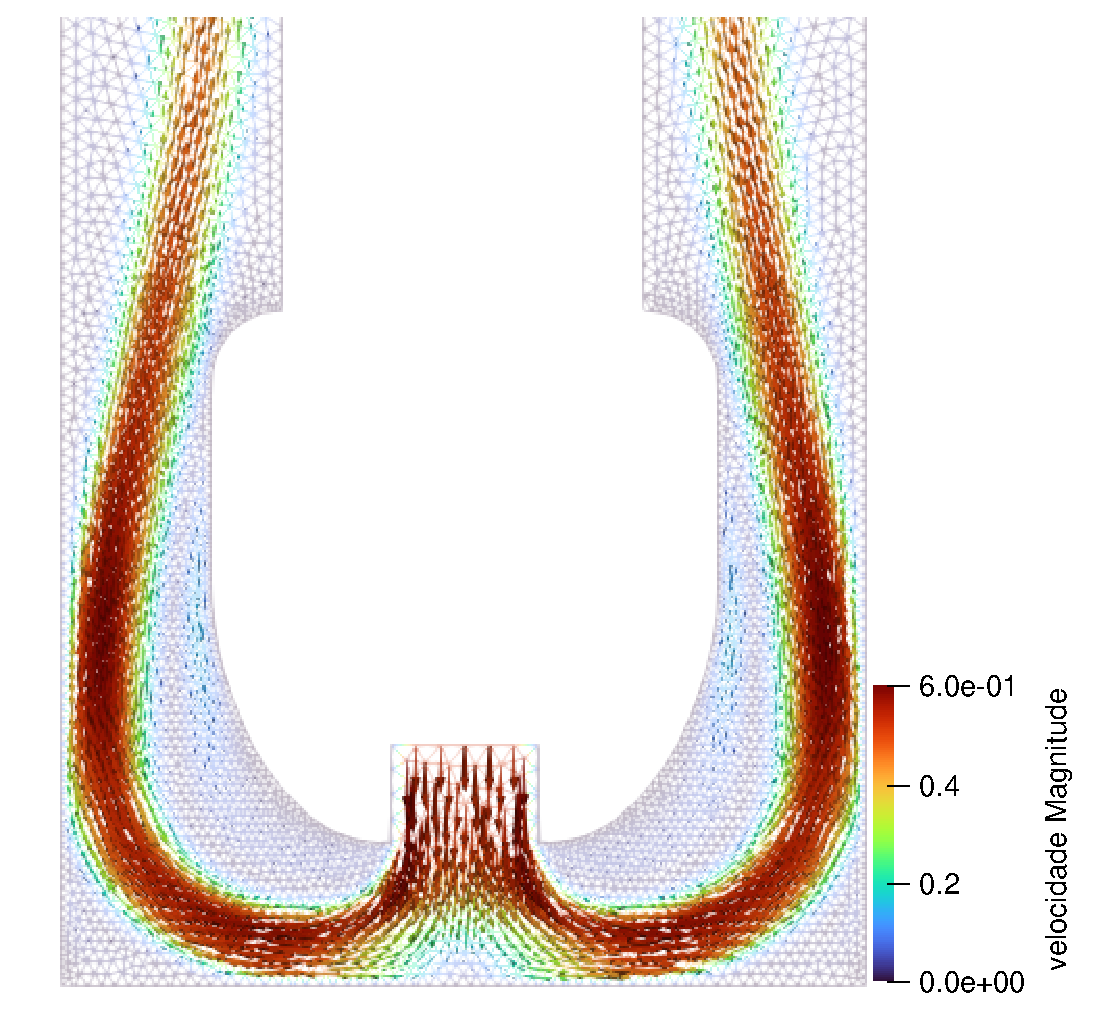
\includegraphics[width=\linewidth]{img/perfil_vel/liso/perfil_de_vel_sapata_paraview_10s.eps}
    	\end{subfigure}
    	
    	\caption{Campo de velocidade na sapata no tempo de 0.5s e 10s na geometria $A_1$. Fonte: autor}
    	\label{fig:perfil_velocidade_liso_sapata_paraview_0_5s}
\end{figure}
    
 A Fig. \ref{fig:perfil_velocidade_liso} mostra o perfil de velocidade na geometria $A_1$ para os 4 níveis distintos.
\begin{figure}[H]
    	\begin{subfigure}[b]{0.42\linewidth}
    		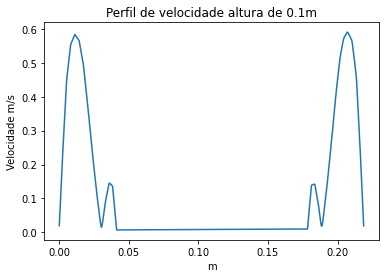
\includegraphics[width=\linewidth]{img/perfil_vel/liso/perfil_velocidade_liso_100.png}
    	\end{subfigure}
    	\begin{subfigure}[b]{0.42\linewidth}
    		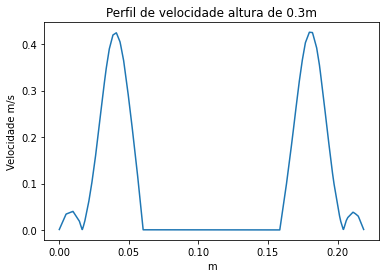
\includegraphics[width=\linewidth]{img/perfil_vel/liso/perfil_velocidade_liso_300.png}
    	\end{subfigure}
    	\\
    	\begin{subfigure}[b]{0.42\linewidth}
    		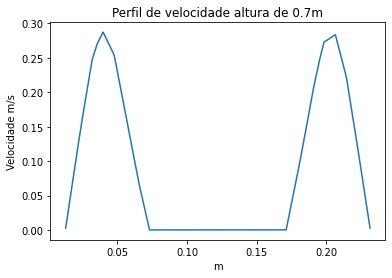
\includegraphics[width=\linewidth]{img/perfil_vel/liso/perfil_velocidade_liso_700.png}
    	\end{subfigure}
    	\begin{subfigure}[b]{0.42\linewidth}
    		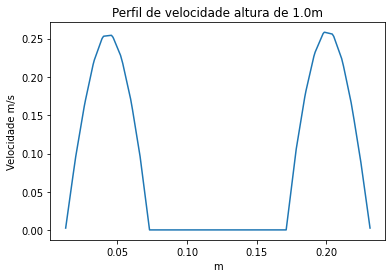
\includegraphics[width=\linewidth]{img/perfil_vel/liso/perfil_velocidade_liso_1000.png}
    	\end{subfigure}
    	\caption{Perfis de velocidade da geometria $A_1$ em 4 níveis distintos}
    	\label{fig:perfil_velocidade_liso}
\end{figure}
    
\begin{comment}
    Cada parâmetro calculado e seus respectivos níveis e lados são especificados na tabela \ref{tab:valor_parametro_A1}.

    \begin{table}[H]
        \centering
        \caption{valor do parâmetro de limpeza para cada nível na geometria $A_1$}
    	\begin{tabular}{ccc}
    		\hline
    		$q$ & $y_k$ & $\eta$ \\
    		\hline
    		E & 0.100 & 0.0744 \\
    		D  & 0.100 & 0.0747 \\
    		E & 0.300 & 0.0125 \\
    		D  & 0.300 & 0.0127 \\
    		E & 0.999 & 0.0274 \\
    		D  & 0.999 & 0.0277 \\
    		\hline
    	\end{tabular}
    	\label{tab:valor_parametro_A1}
    \end{table}
\end{comment}
    
Considerando agora a geometria $A_2$, de parede lisa e valor de \textit{standoff} de 50\%, o campo de velocidade na saída é mostrado na Fig. \ref{fig:perfil_velocidade_liso_saida_standoff_paraview}.
\begin{figure}[H]
        \centering
    	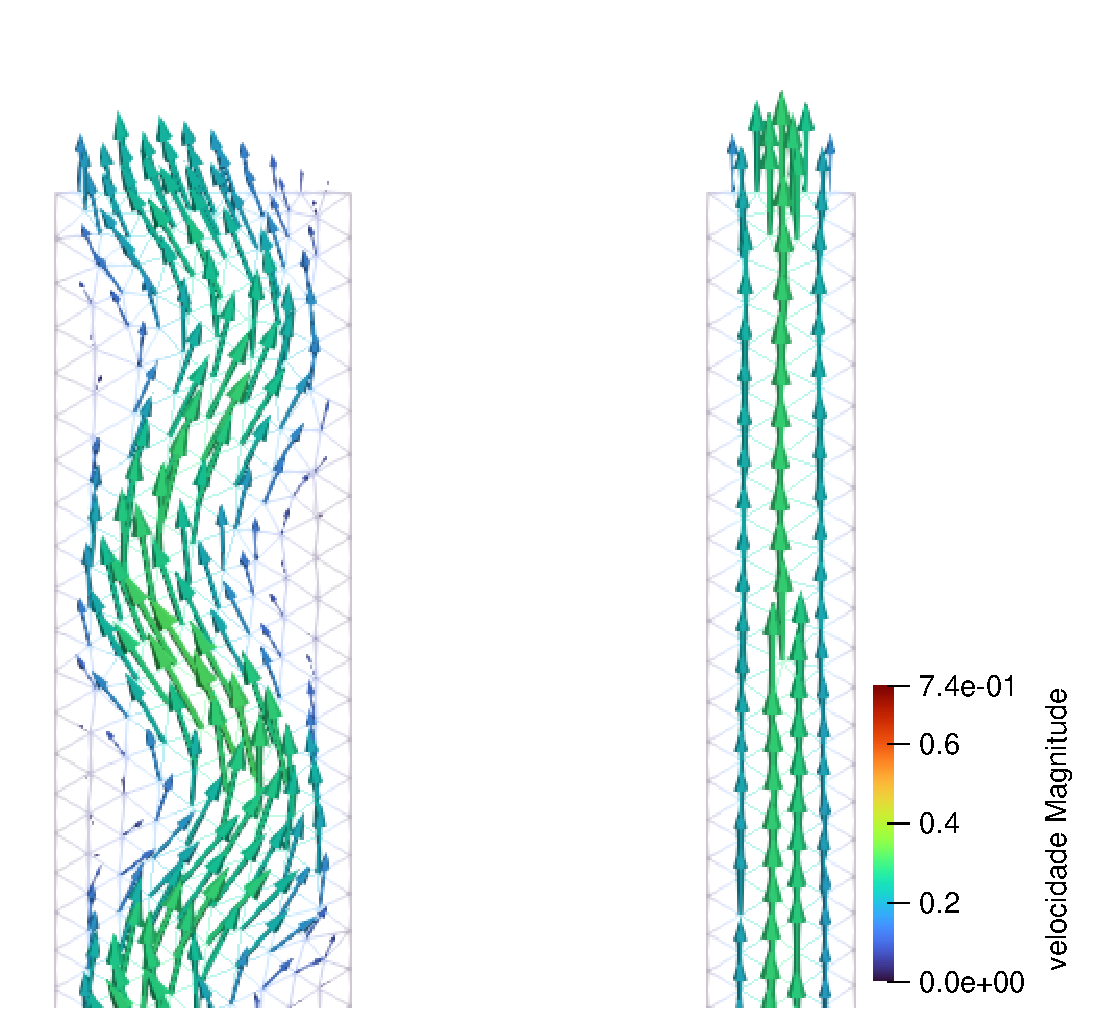
\includegraphics[scale=0.5]{img/perfil_vel/liso/perfil_de_vel_saida_standoff_paraview.eps}
    	\caption{Campo de velocidade na saída do espaço anular no tempo de 10s na geometria $A_2$. Fonte: autor}
    	\label{fig:perfil_velocidade_liso_saida_standoff_paraview}
\end{figure}
    
É evidente o efeito do standoff no escoamento, o fluxo teve um comportamento ondulatório. Na região da sapata, perto do fundo do poço Fig. \ref{fig:perfil_velocidade_liso_sapata_standoff_paraview_0_5s} é possível observar que do lado direito a velocidade teve um perfil mais regular que do lado esquerdo. 
     
\begin{figure}[H]
        \centering
        \begin{subfigure}[b]{0.42\linewidth}
    		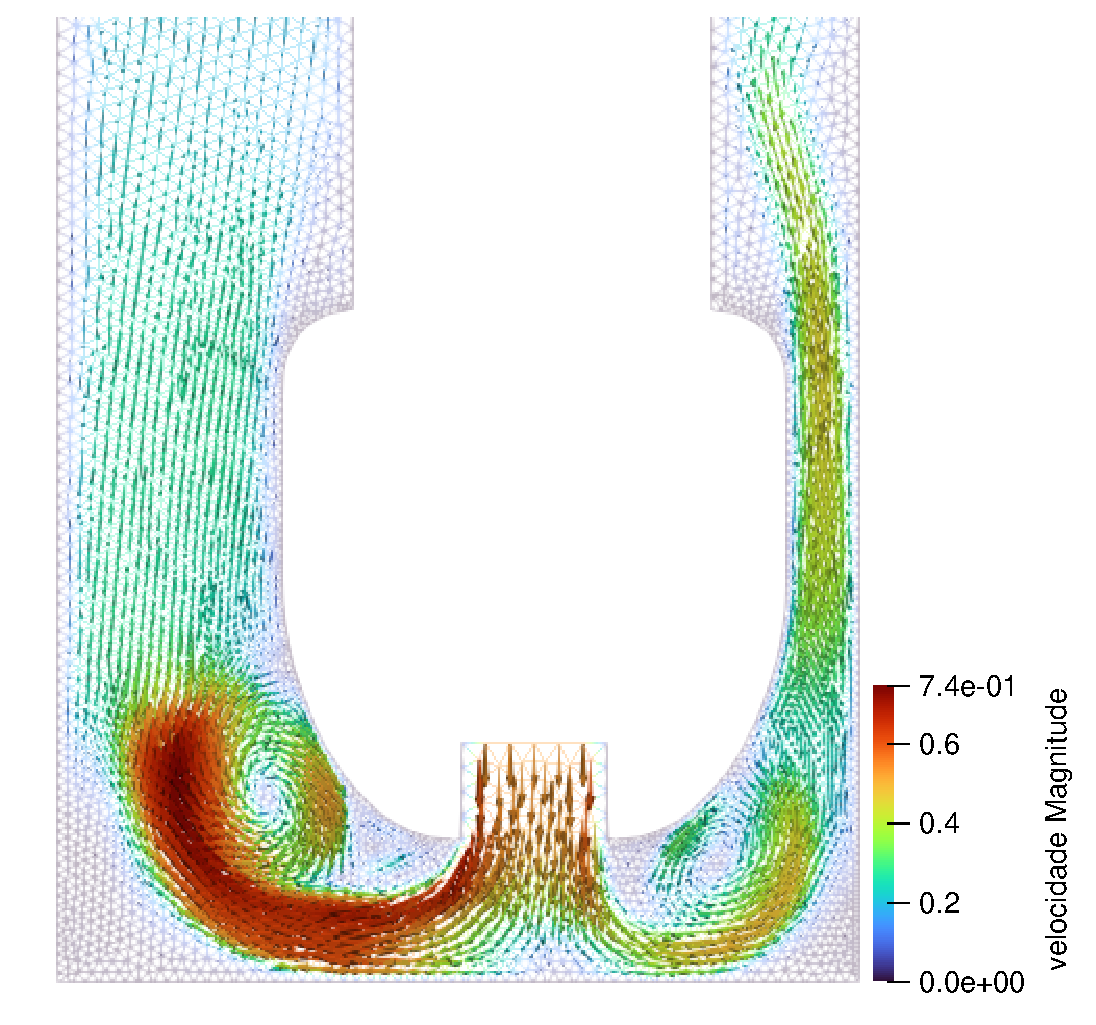
\includegraphics[width=\linewidth]{img/perfil_vel/liso/perfil_de_vel_sapata_standoff_paraview_0.5s.eps}
    	\end{subfigure}
    	\begin{subfigure}[b]{0.42\linewidth}
    		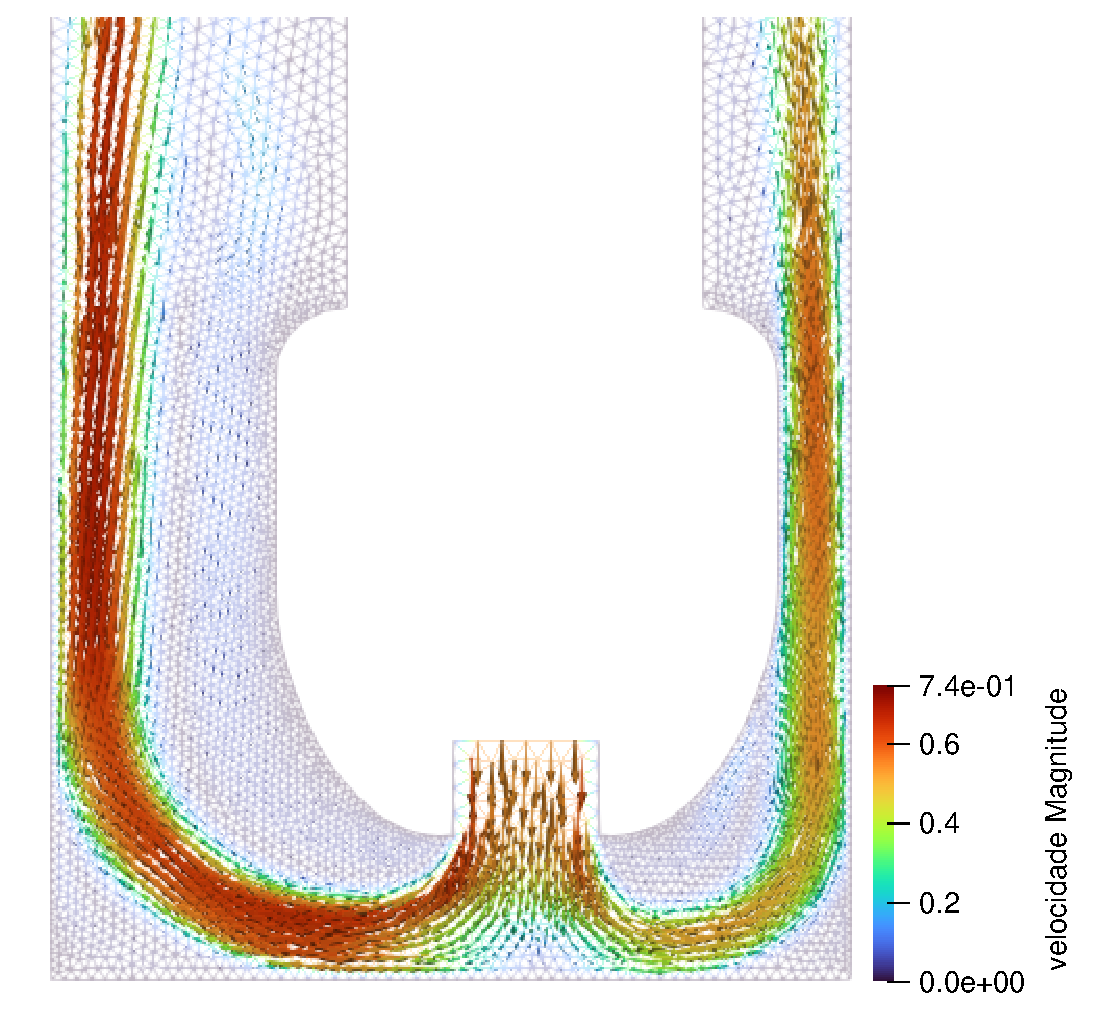
\includegraphics[width=\linewidth]{img/perfil_vel/liso/perfil_de_vel_sapata_standoff_paraview_10s.eps}
    	\end{subfigure}
    	\caption{Campo de velocidade na sapata no tempo de 0.5s e 10s na geometria $A_2$. Fonte: autor}
    	\label{fig:perfil_velocidade_liso_sapata_standoff_paraview_0_5s}
\end{figure}
    
Os perfis de velocidade para os 4 níveis selecionados na geometria onde não há nenhuma rugosidade na parede do poço e um valor de \textit{standoff} menor que 100\% podem ser visualizados na figura 
\begin{figure}[H]
    	\begin{subfigure}[b]{0.42\linewidth}
    		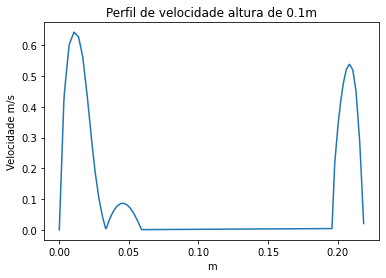
\includegraphics[width=\linewidth]{img/perfil_vel/liso/perfil_velocidade_liso_s_100.png}
    	\end{subfigure}
    	\begin{subfigure}[b]{0.42\linewidth}
    		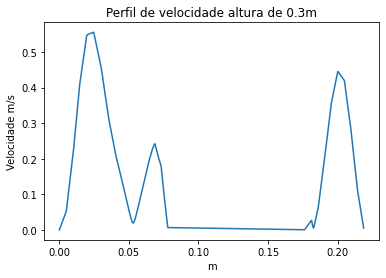
\includegraphics[width=\linewidth]{img/perfil_vel/liso/perfil_velocidade_liso_s_300.png}
    	\end{subfigure}
    	\\
    	\begin{subfigure}[b]{0.42\linewidth}
    		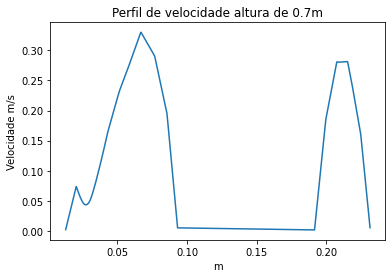
\includegraphics[width=\linewidth]{img/perfil_vel/liso/perfil_velocidade_liso_s_700.png}
    	\end{subfigure}
    	\begin{subfigure}[b]{0.42\linewidth}
    		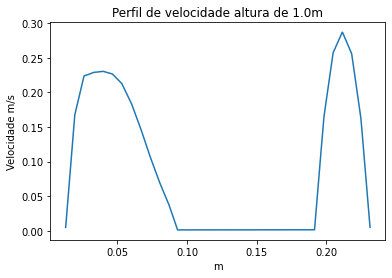
\includegraphics[width=\linewidth]{img/perfil_vel/liso/perfil_velocidade_liso_s_1000.png}
    	\end{subfigure}
    	\caption{Perfis de velocidade da geometria $A_2$ em 4 níveis distintos}
    	\label{fig:perfil_velocidade_liso_standoff}
\end{figure}
    
Recortes do campo de pressão das geometrias $A$ podem ser vistos na Fig. \ref{fig:cpressaoA1A2}
\begin{figure}[H]
        \centering
        \begin{subfigure}[b]{0.42\linewidth}
    		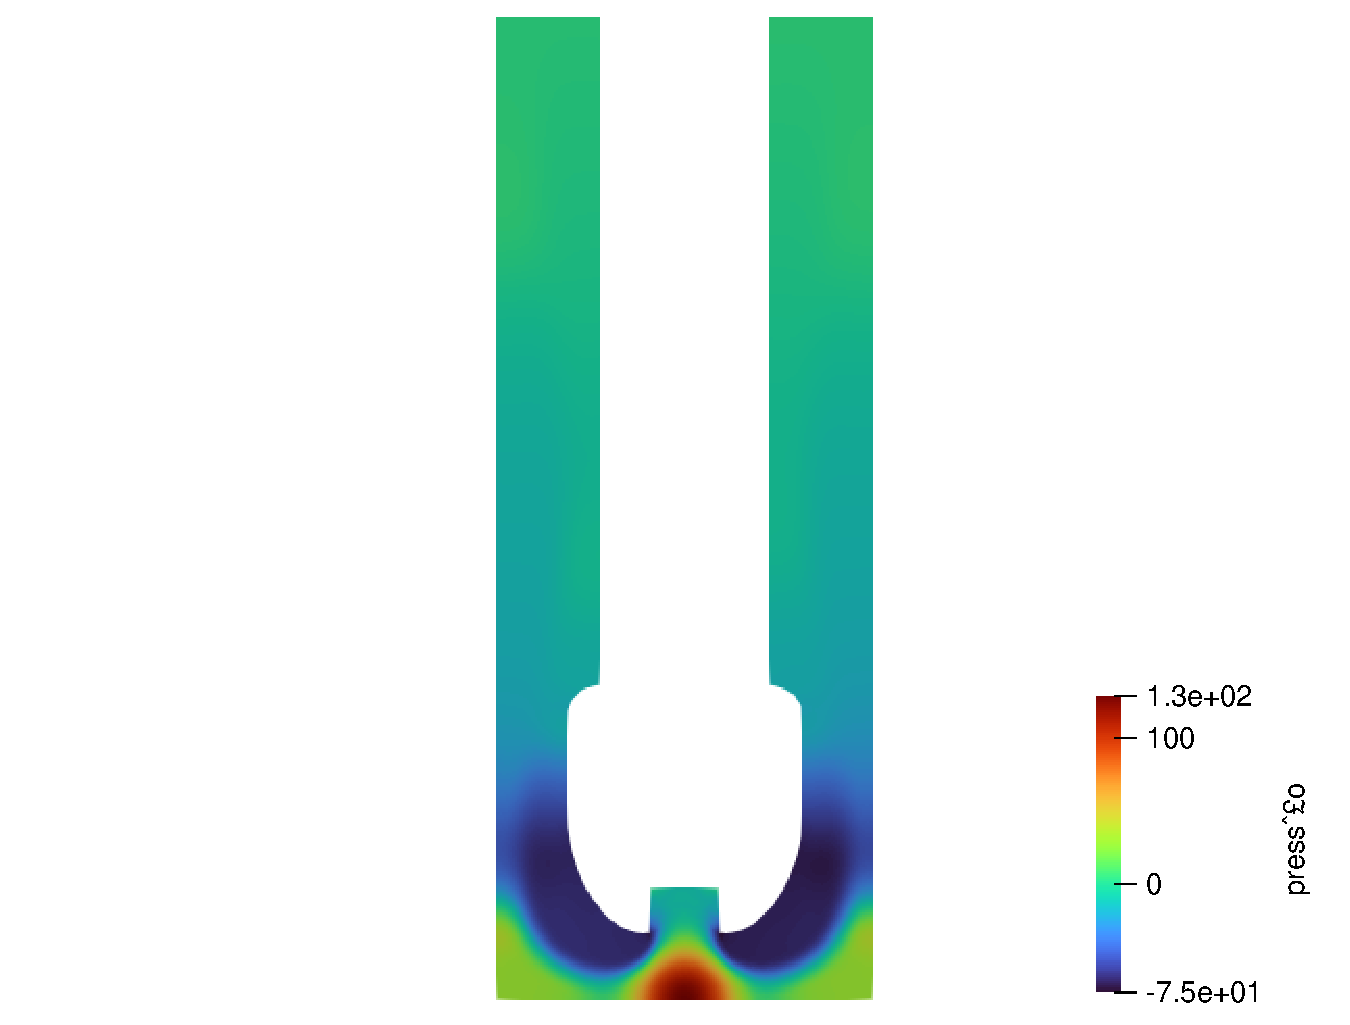
\includegraphics[width=\linewidth]{img/campo_press/liso/campo_de_pres_paraview.eps}
    	\end{subfigure}
    	\begin{subfigure}[b]{0.42\linewidth}
    		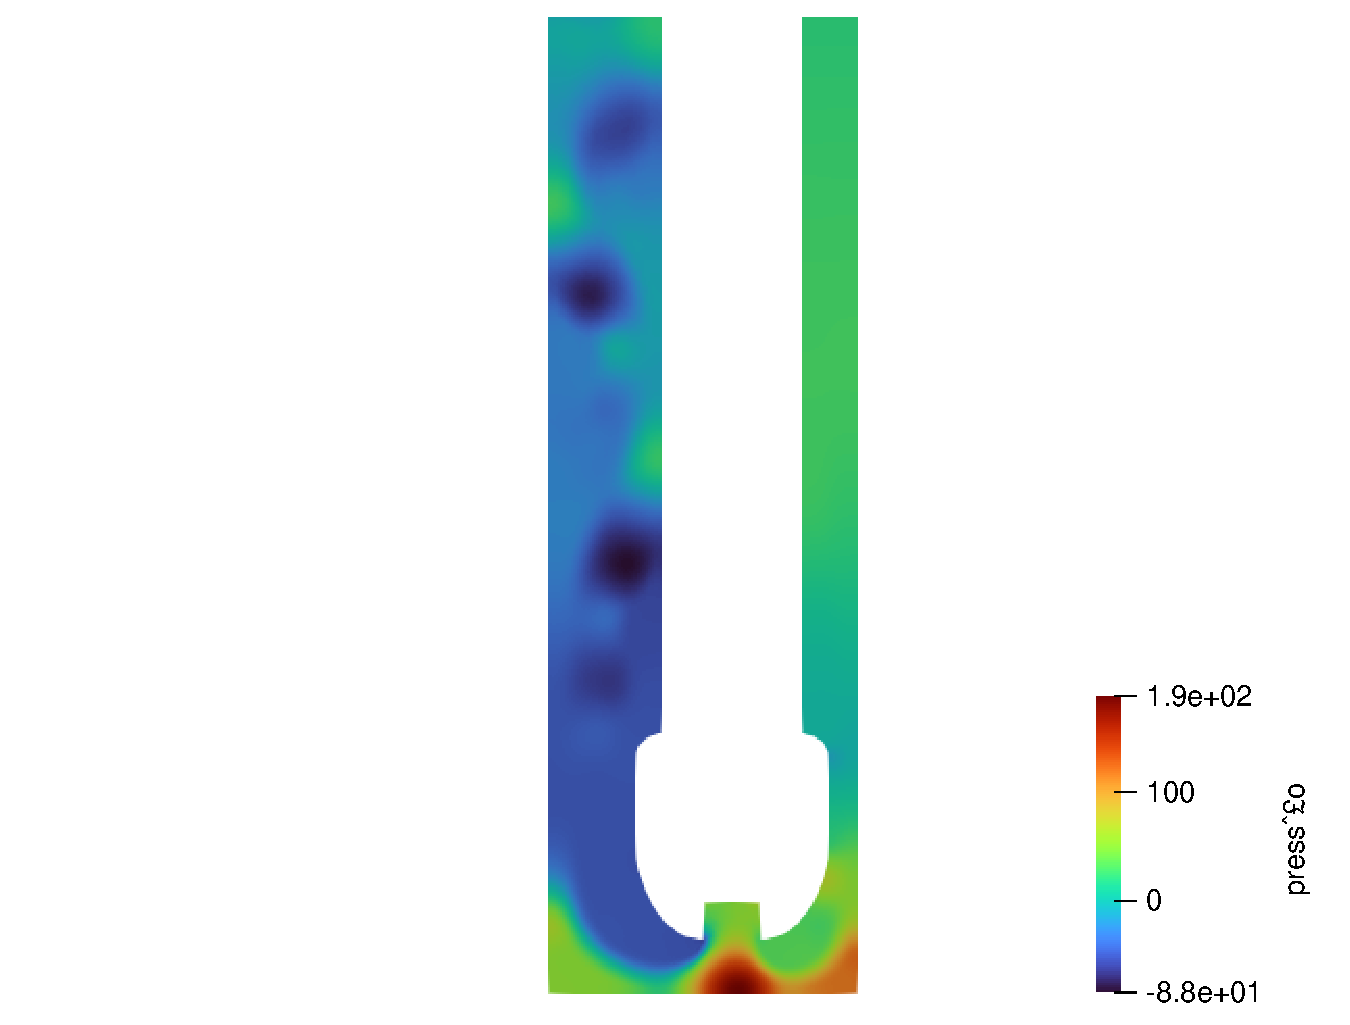
\includegraphics[width=\linewidth]{img/campo_press/liso/campo_de_pres_standoff_paraview.eps}
    	\end{subfigure}
    	\caption{Campo de pressão nas geometrias $A$. Fonte: autor}
    	\label{fig:cpressaoA1A2}
\end{figure}
    
\begin{comment}
    Cada parâmetro calculado e seus respectivos níveis e lados são especificados na tabela \ref{tab:valor_parametro_A2}.
    
    \begin{table}[H]
        \centering
        \caption{valor do parâmetro de limpeza para cada nível na geometria $A_2$}
    	\begin{tabular}{ccc}
    		\hline
    		$q$ & $y_k$ & $\eta$ \\
    		\hline
    		E & 0.100 & 0.0744 \\
    		D  & 0.100 & 0.0747 \\
    		E & 0.300 & 0.0125 \\
    		D  & 0.300 & 0.0127 \\
    		E & 0.999 & 0.0274 \\
    		D  & 0.999 & 0.0277 \\
    		\hline
    	\end{tabular}
    	\label{tab:valor_parametro_A2}
    \end{table}
\end{comment}


\subsubsection{Configurações com Erosões}
    
Para o caso das geometrias $B$, em que há um certo grau de erosão na parede da formação, o perfil de velocidade na saída do anular observado na Fig. \ref{fig:perfil_velocidade_rugoso_saida_paraview_10s} mostra um escoamento parabólico. O mesmo comportamento foi visto nas geometrias $A$. Logo, a erosão não causou interferências.
\begin{figure}[H]
        \centering
    	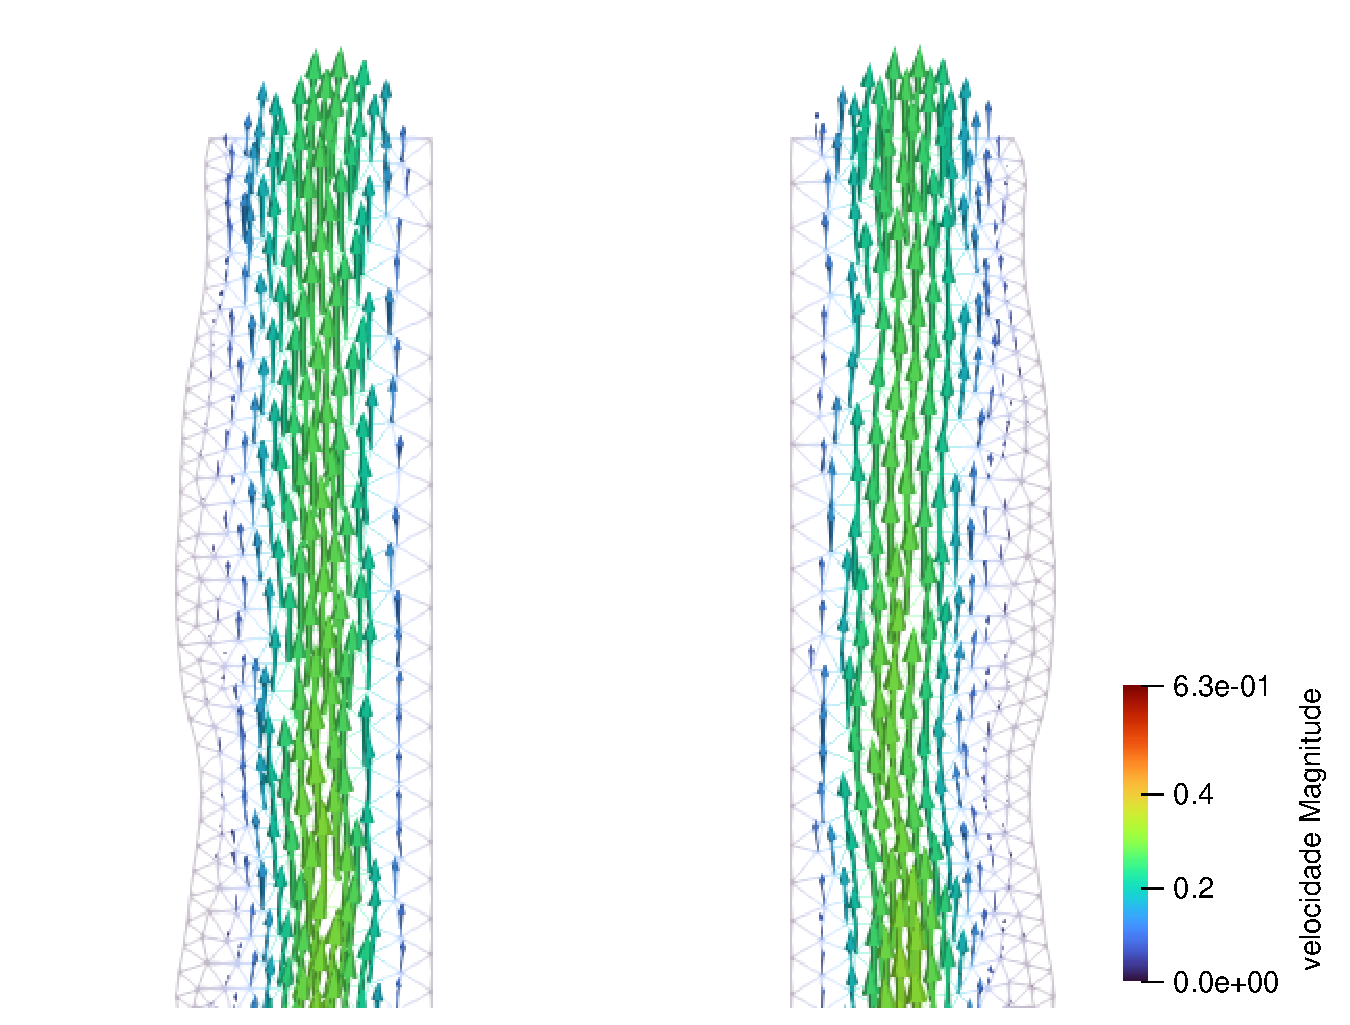
\includegraphics[scale=0.5]{img/perfil_vel/rugoso/perfil_de_vel_saida_paraview.eps}
    	\caption{Campo de velocidade na saída do espaço anular no tempo de 10s na geometria $B_1$. Fonte: autor}
    	\label{fig:perfil_velocidade_rugoso_saida_paraview_10s}
\end{figure}
    
A Fig. \ref{fig:perfil_velocidade_rugoso_sapata_paraview_0.5s} mostra o comportamento do fluido na sapata no tempo de $0.5s$ e $10s$ evidenciando o efeito da erosão se comparado a Fig. \ref{fig:perfil_velocidade_liso_sapata_paraview_0_5s} pode-se observar que o comportamento do fluido foi simétrico como na geometria $A_1$ e concluir que o efeito da erosão nesse caso não teve impacto expressivo
    
    \begin{figure}[H]
        \centering
        \begin{subfigure}[b]{0.42\linewidth}
            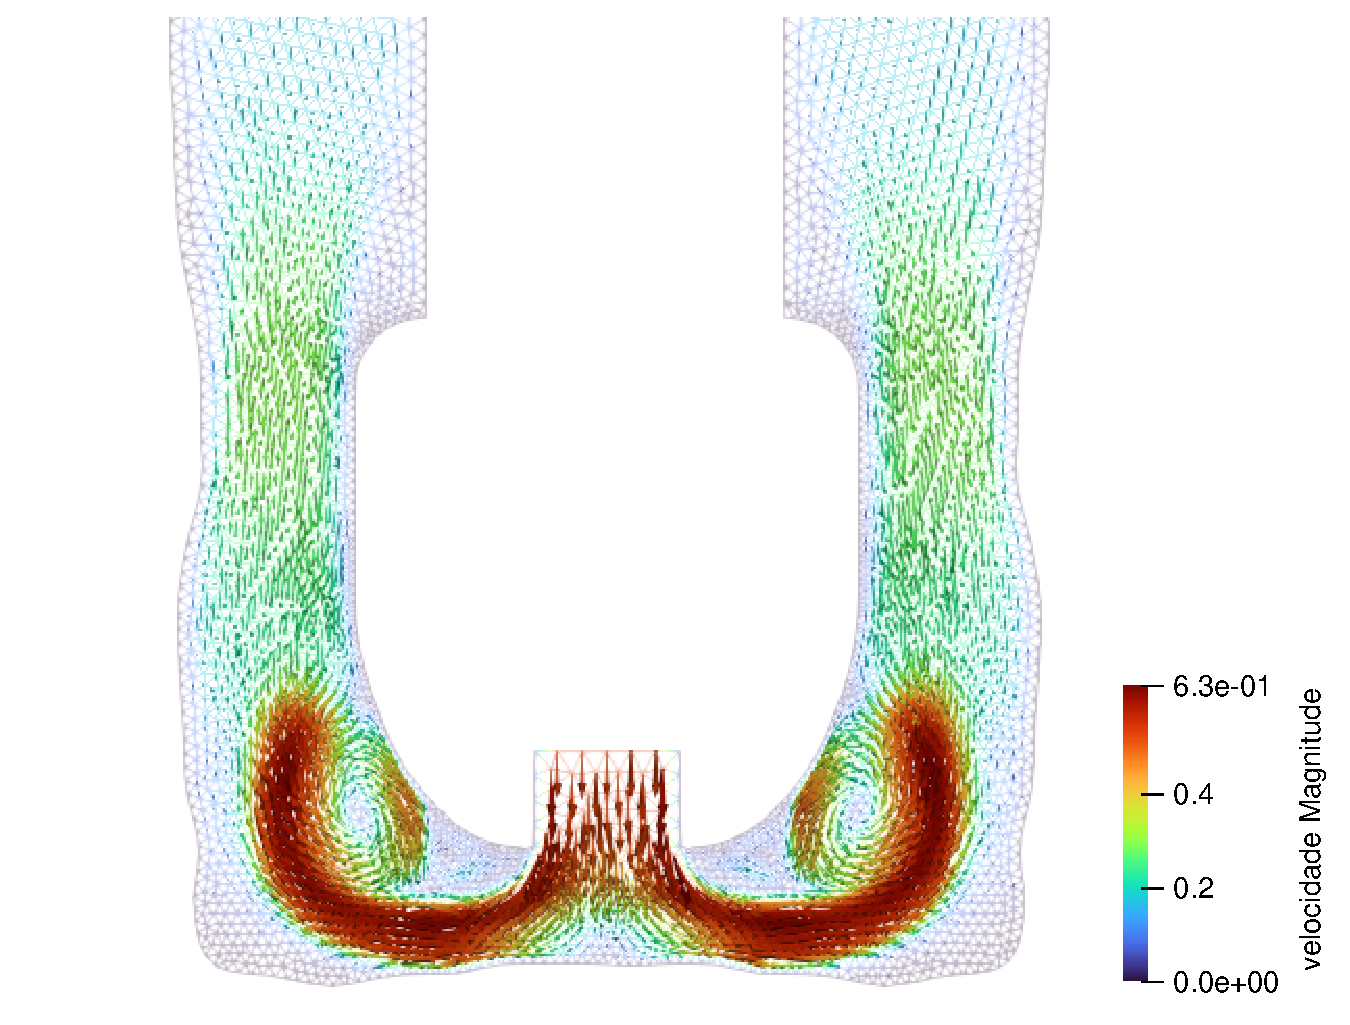
\includegraphics[width=\linewidth]{img/perfil_vel/rugoso/perfil_de_vel_sapata_paraview_0.5s.eps}
        \end{subfigure}
        \begin{subfigure}[b]{0.42\linewidth}
            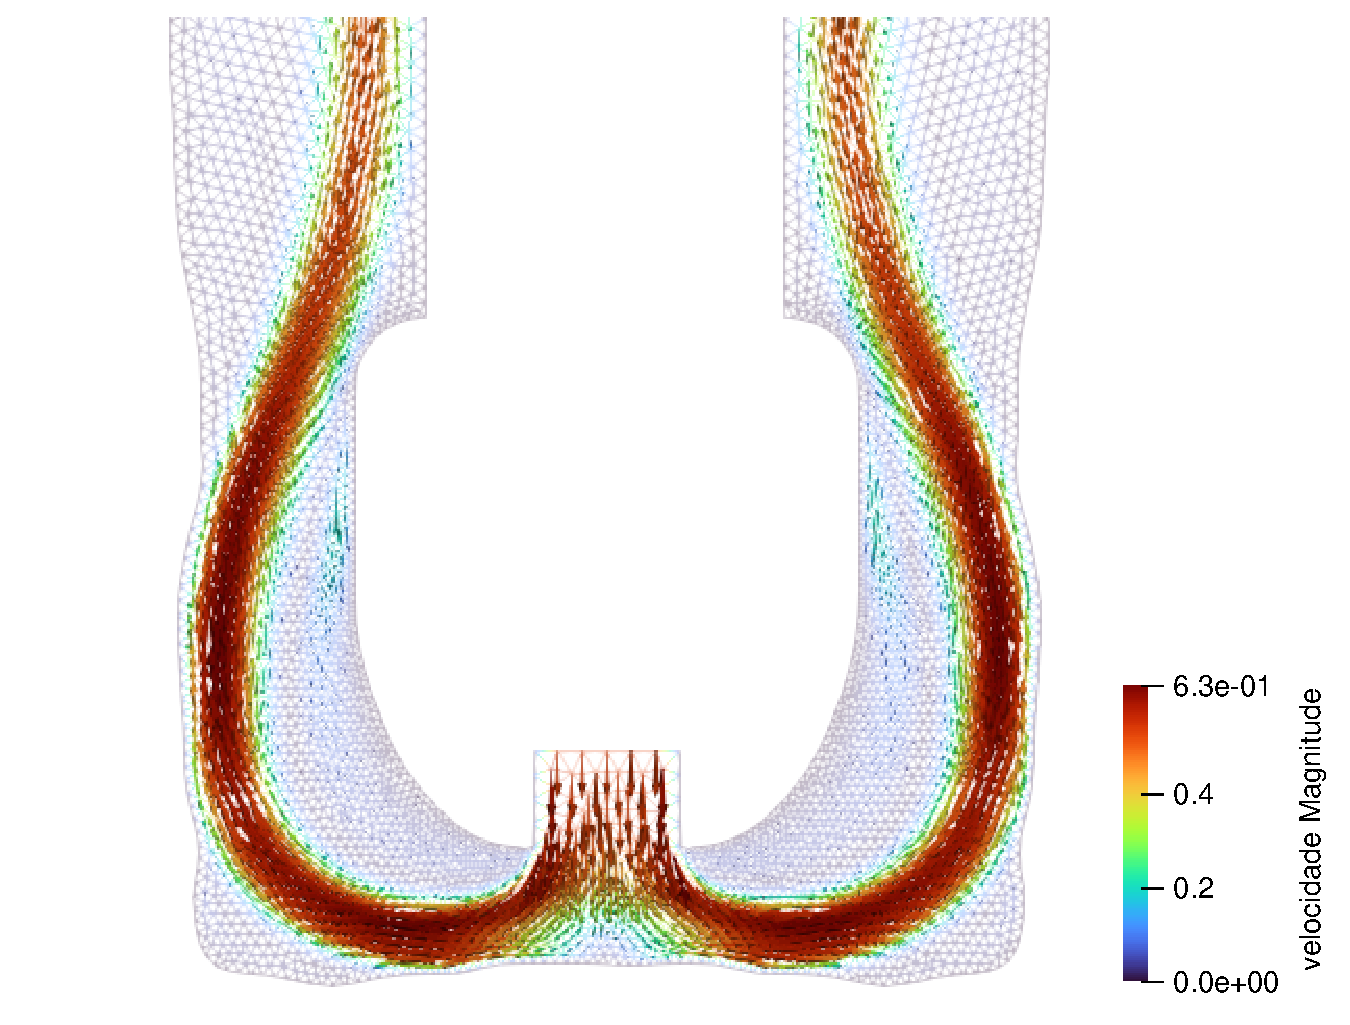
\includegraphics[width=\linewidth]{img/perfil_vel/rugoso/perfil_de_vel_sapata_paraview_10s.eps}
        \end{subfigure}
    	
    	\caption{Campo de velocidade na sapata no tempo de 0.5s e 10s na geometria $B_1$. Fonte: autor}
    	\label{fig:perfil_velocidade_rugoso_sapata_paraview_0.5s}
    \end{figure}
    
Os perfis de velocidade para os 4 níveis selecionados na geometria onde há rugosidade na parede do poço e um valor de \textit{standoff} igual a 100\% ($B_1$) podem ser visualizados na figura \ref{fig:perfil_velocidade_rugosa}.
    \begin{figure}[H]
        \centering
    	\begin{subfigure}[b]{0.42\linewidth}
    		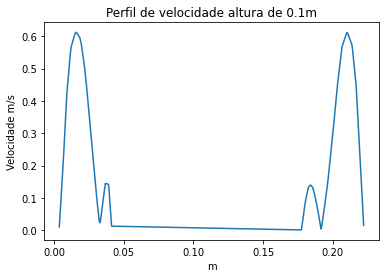
\includegraphics[width=\linewidth]{img/perfil_vel/rugoso/perfil_velocidade_rugoso_100.png}
    	\end{subfigure}
    	\begin{subfigure}[b]{0.42\linewidth}
    		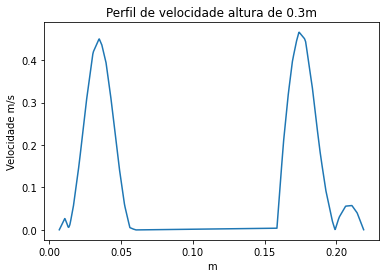
\includegraphics[width=\linewidth]{img/perfil_vel/rugoso/perfil_velocidade_rugoso_300.png}
    	\end{subfigure}
    	\\
    	\begin{subfigure}[b]{0.42\linewidth}
    		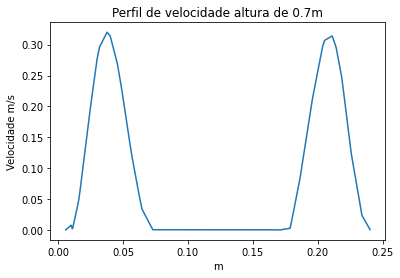
\includegraphics[width=\linewidth]{img/perfil_vel/rugoso/perfil_velocidade_rugoso_700.png}
    	\end{subfigure}
    	\begin{subfigure}[b]{0.42\linewidth}
    		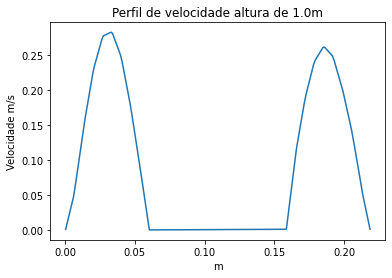
\includegraphics[width=\linewidth]{img/perfil_vel/rugoso/perfil_velocidade_rugoso_1000.png}
    	\end{subfigure}
    	\caption{Perfis de velocidade da geometria $B_1$ em 4 níveis distintos}
    	\label{fig:perfil_velocidade_rugosa}
    \end{figure}
    
\begin{comment}
    Cada parâmetro calculado e seus respectivos níveis e lados são especificados na tabela \ref{tab:valor_parametro_B1}.
    
    \begin{table}[H]
        \centering
        \caption{valor do parâmetro de limpeza para cada nível na geometria $B_1$}
    	\begin{tabular}{ccc}
    		\hline
    		$q$ & $y_k$ & $\eta$ \\
    		\hline
    		E & 0.100 & 0.0744 \\
    		D  & 0.100 & 0.0747 \\
    		E & 0.300 & 0.0125 \\
    		D  & 0.300 & 0.0127 \\
    		E & 0.999 & 0.0274 \\
    		D  & 0.999 & 0.0277 \\
    		\hline
    	\end{tabular}
    	\label{tab:valor_parametro_B1}
    \end{table}
\end{comment}
   
Para o caso da geometria $B_2$, onde a taxa de \textit{standoff} é de 50\%, o perfil de velocidade na saída do anular observado na Fig. \ref{fig:perfil_velocidade_rugoso_saida_paraview_10s} mostra um escoamento parabólico, esse mesmo comportamento foi visto nas geometrias $A$, portanto, a erosão não causou interferência nesse sentido, porém a erosão causou um efeito de irregularidade no escoamento com pequenas zonas de recirculação.
    
\begin{figure}[H]
        \centering
    	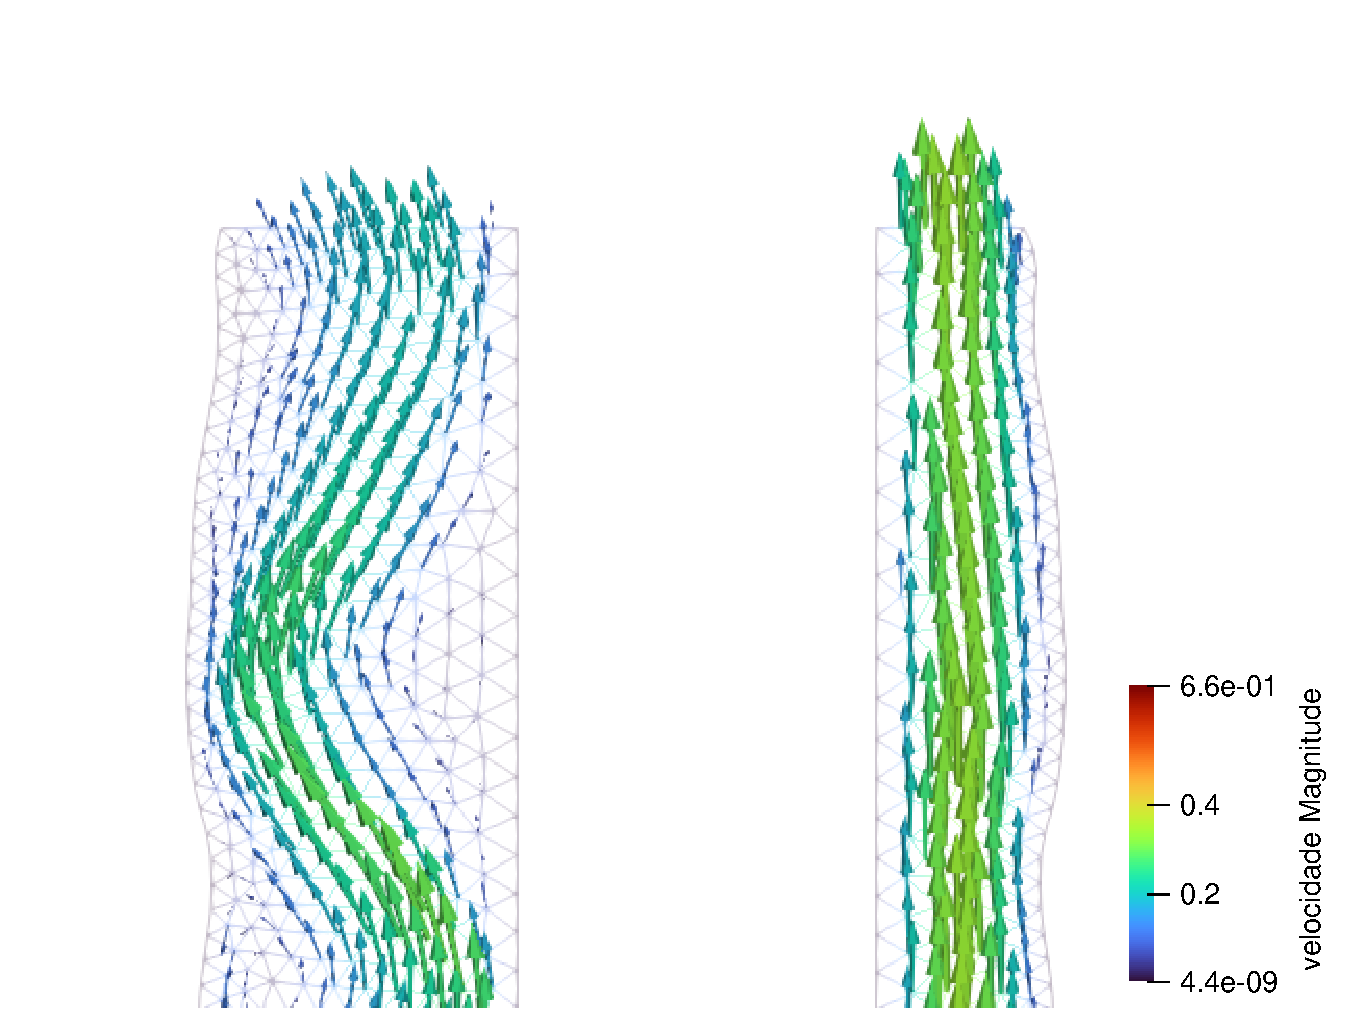
\includegraphics[scale=0.5]{img/perfil_vel/rugoso/perfil_de_vel_saida_standoff_paraview.eps}
    	\caption{Campo de velocidade na saída do espaço anular no tempo de 10s na geometria $B_2$. Fonte: autor}
    	\label{fig:perfil_velocidade_rugoso_saida_paraview_10s}
\end{figure}
    
A Fig. \ref{fig:perfil_velocidade_rugoso_sapata_standoff_paraview_0.5s} mostra o comportamento do fluido na sapata nos tempos de $0.5s$ e $10s$ evidenciando o efeito da erosão se comparado a Fig. \ref{fig:perfil_velocidade_liso_sapata_standoff_paraview_0_5s} pode-se observar que o comportamento do fluido não foi simétrico como na geometria $A_2$
    \begin{figure}[H]
        \centering
        \begin{subfigure}[b]{0.42\linewidth}
            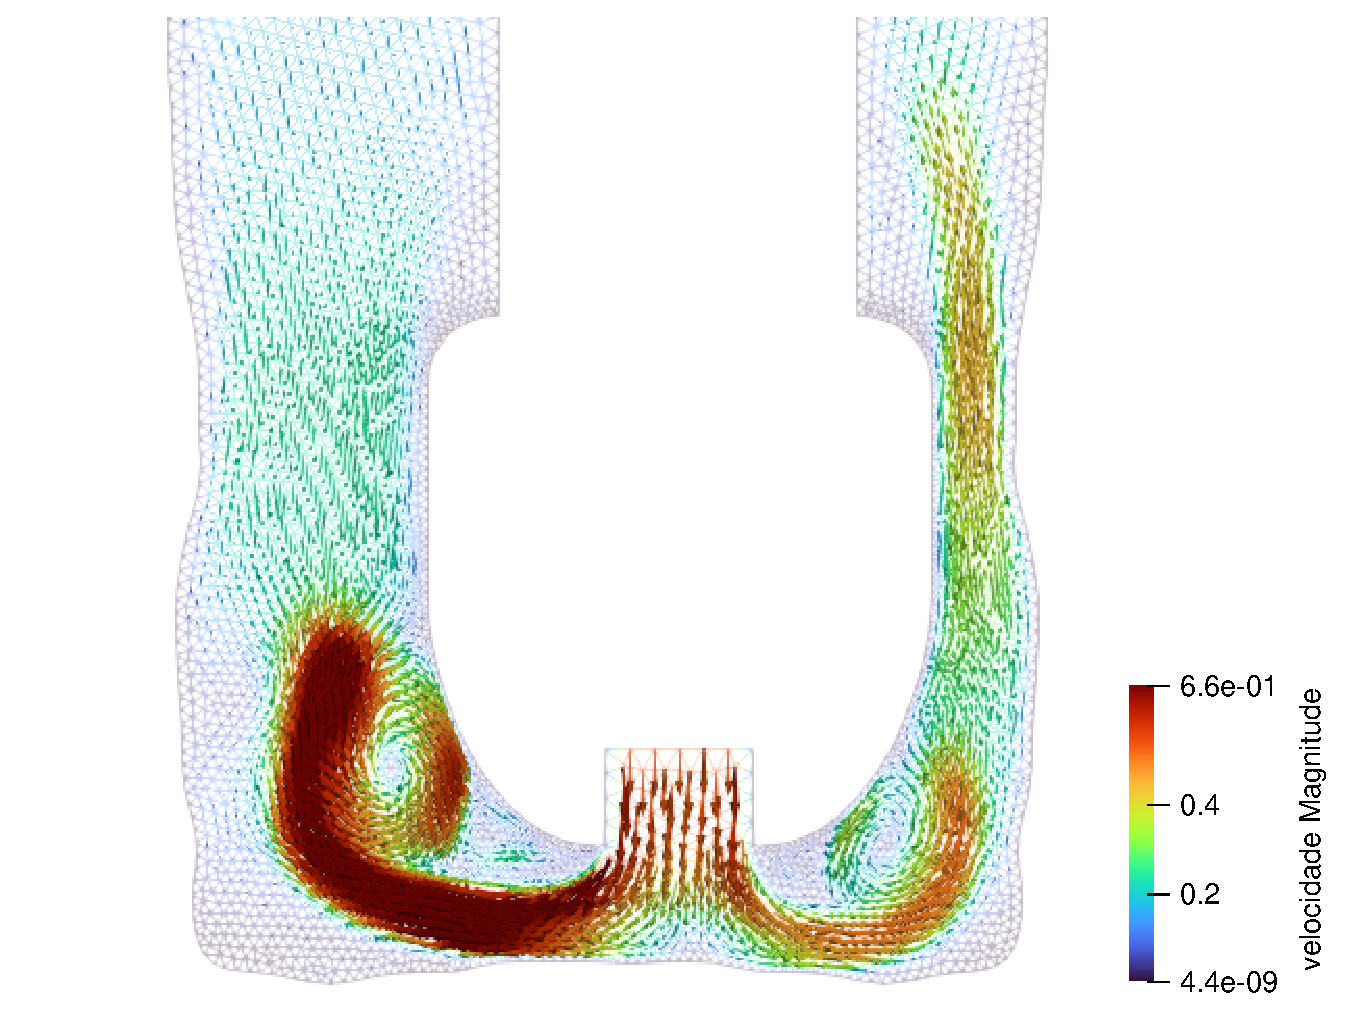
\includegraphics[width=\linewidth]{img/perfil_vel/rugoso/perfil_de_vel_sapata_standoff_paraview_0_5s.eps}
        \end{subfigure}
        \begin{subfigure}[b]{0.42\linewidth}
            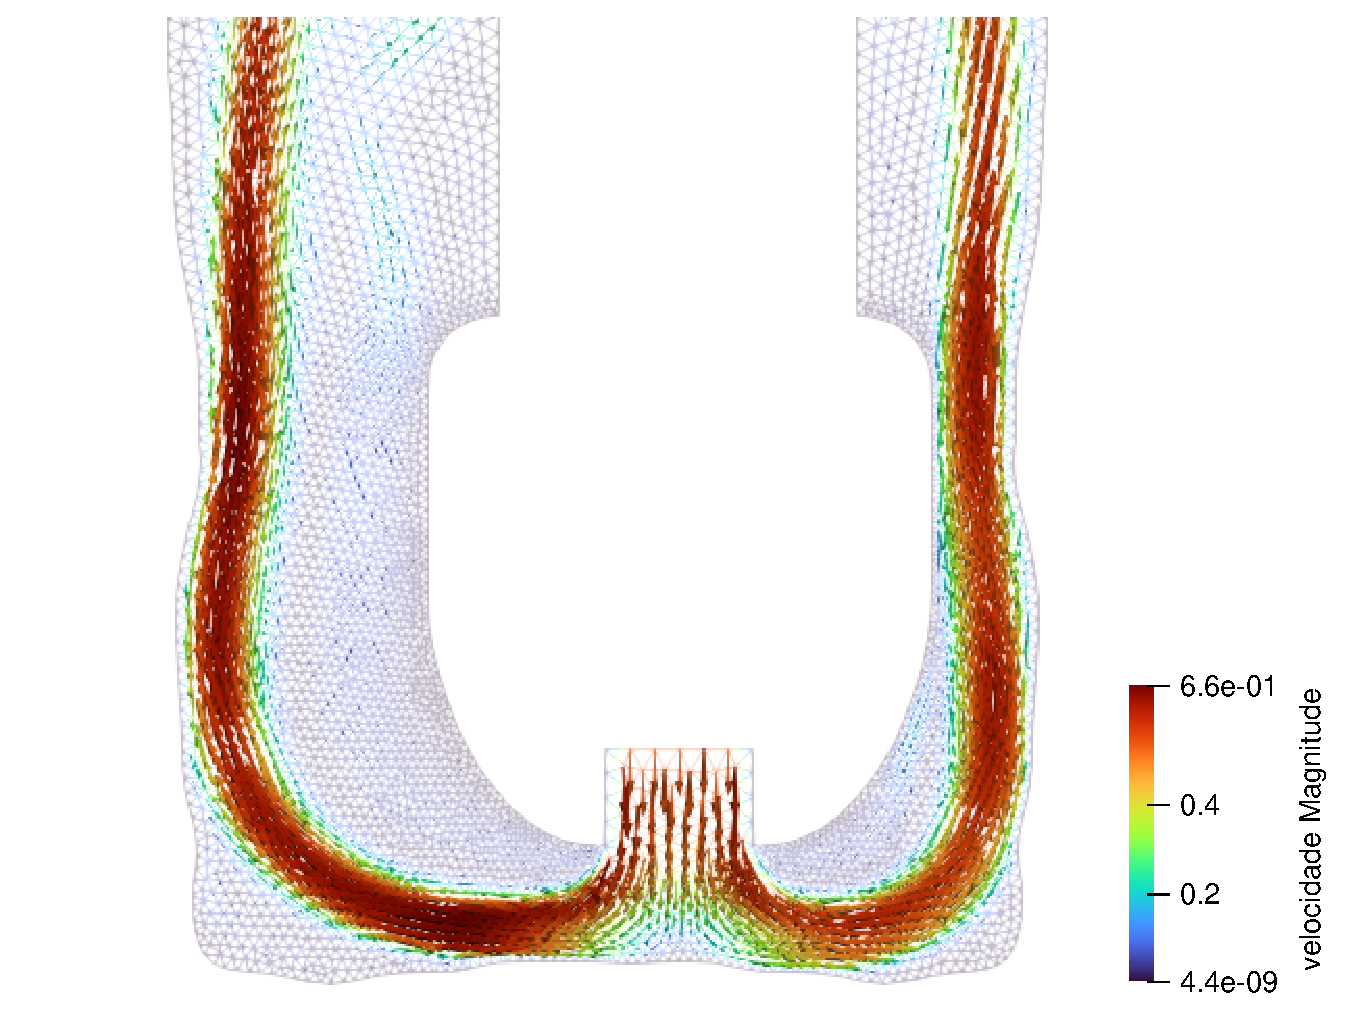
\includegraphics[width=\linewidth]{img/perfil_vel/rugoso/perfil_de_vel_sapata_standoff_paraview_10s.eps}
        \end{subfigure}
    	
    	\caption{Campo de velocidade na sapata no tempo de 0.5s e $10s$ na geometria $B_2$. Fonte: autor}
    	\label{fig:perfil_velocidade_rugoso_sapata_standoff_paraview_0.5s}
    \end{figure}
    
Os perfis de velocidade para os 4 níveis selecionados na geometria onde há rugosidade na parede do poço e um valor de \textit{standoff} menor que 100\% $B_2$ podem ser visualizado na figura \ref{fig:perfil_velocidade_rugosa_standoff}.
    \begin{figure}[H]
    	\begin{subfigure}[b]{0.42\linewidth}
    		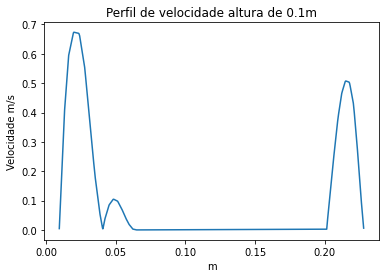
\includegraphics[width=\linewidth]{img/perfil_vel/rugoso/perfil_velocidade_rugoso_s_100.png}
    	\end{subfigure}
    	\begin{subfigure}[b]{0.42\linewidth}
    		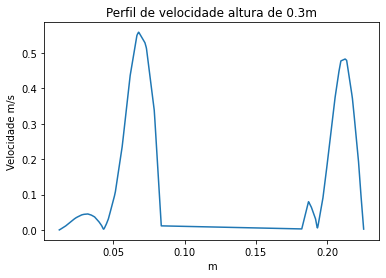
\includegraphics[width=\linewidth]{img/perfil_vel/rugoso/perfil_velocidade_rugoso_s_300.png}
    	\end{subfigure}
    	\\
    	\begin{subfigure}[b]{0.42\linewidth}
    		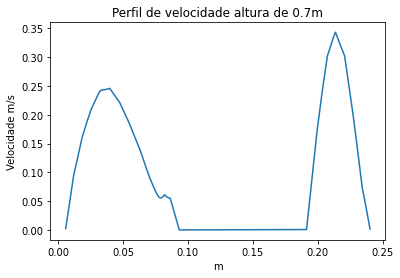
\includegraphics[width=\linewidth]{img/perfil_vel/rugoso/perfil_velocidade_rugoso_s_700.png}
    	\end{subfigure}
    	\begin{subfigure}[b]{0.42\linewidth}
    		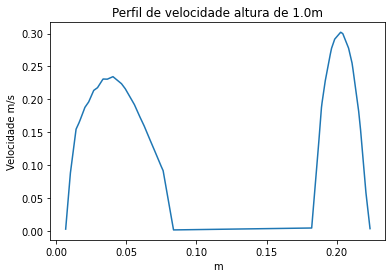
\includegraphics[width=\linewidth]{img/perfil_vel/rugoso/perfil_velocidade_rugoso_s_1000.png}
    	\end{subfigure}
    	\caption{Perfis de velocidade da geometria $B_2$ para 4 níveis distintos}
    	\label{fig:perfil_velocidade_rugosa_standoff}
    \end{figure}
    
Recortes do campo de pressão das geometrias $B$ podem ser vistos na Fig. \ref{fig:cpressaoB1B2}.
\begin{figure}[H]
        \centering
        \begin{subfigure}[b]{0.42\linewidth}
    		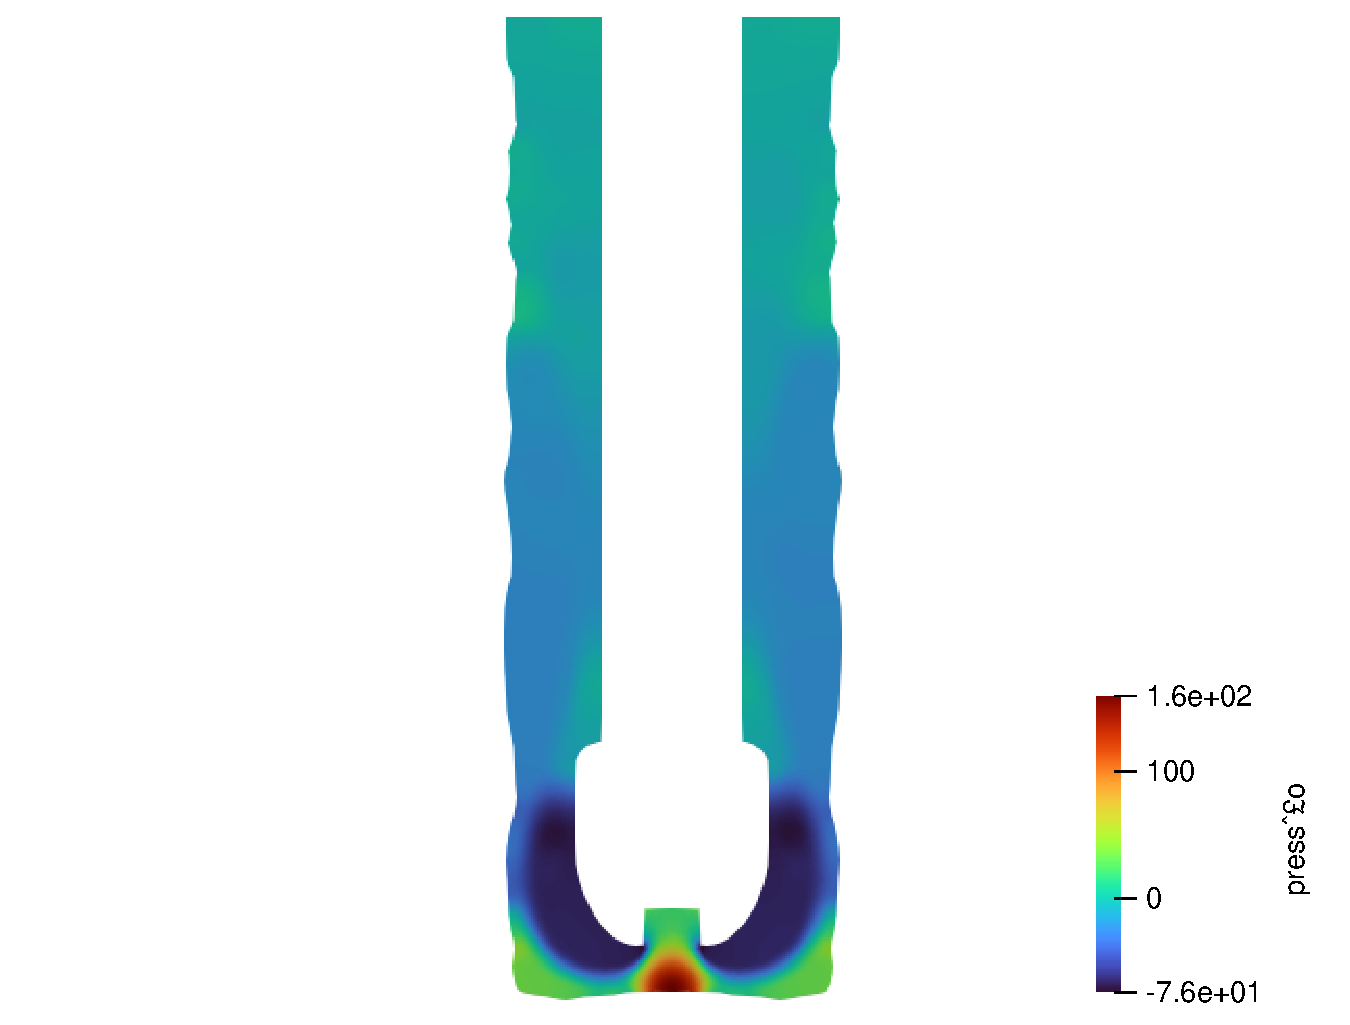
\includegraphics[width=\linewidth]{img/campo_press/rugoso/campo_de_pres_paraview.eps}
    	\end{subfigure}
    	\begin{subfigure}[b]{0.42\linewidth}
    		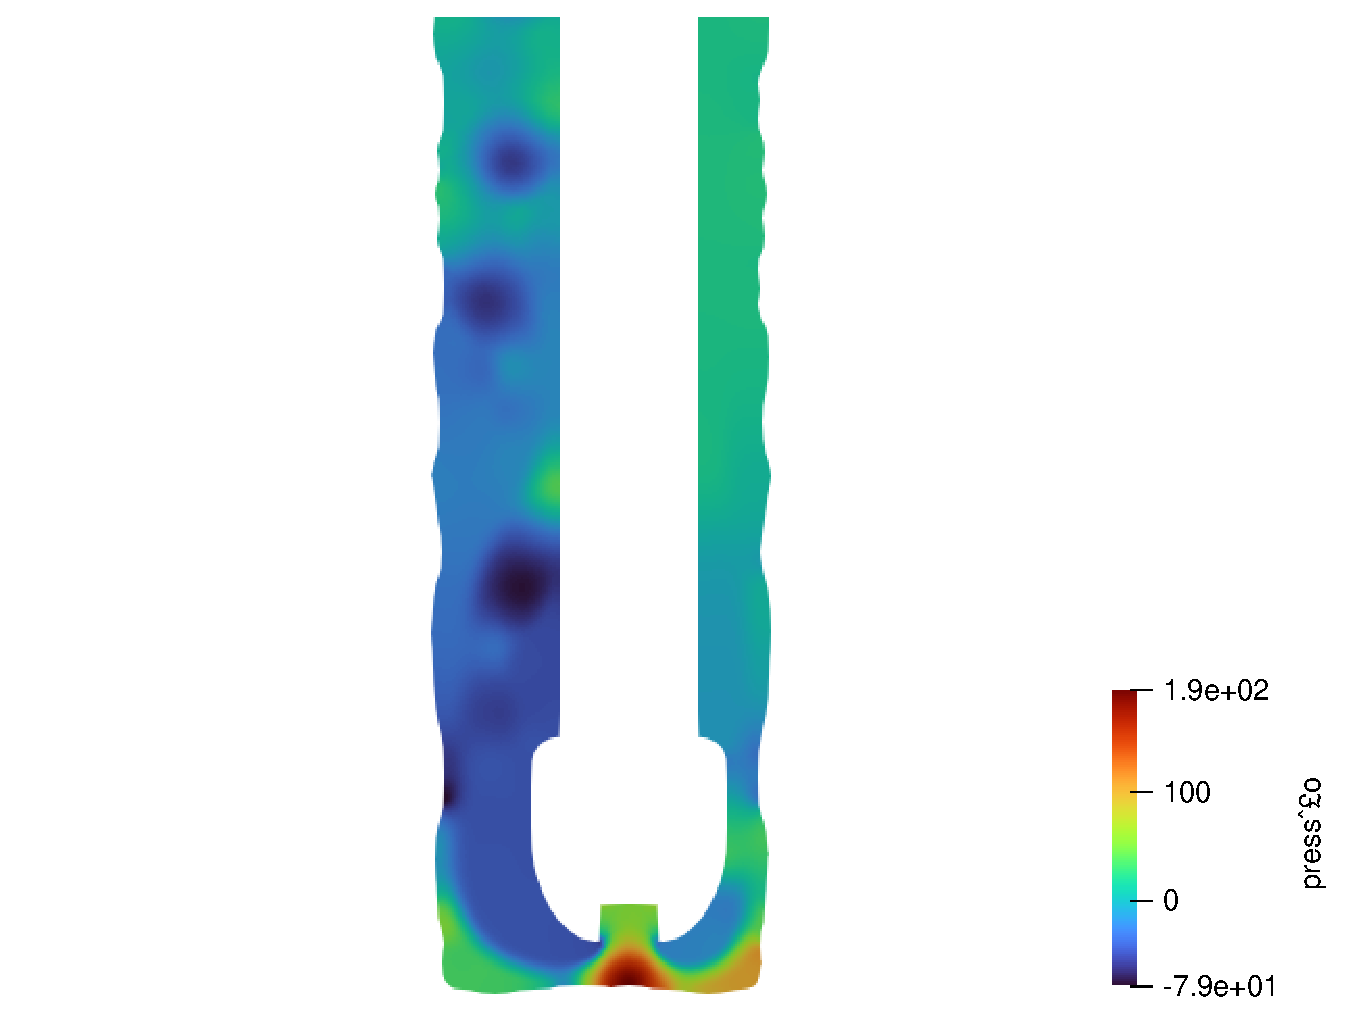
\includegraphics[width=\linewidth]{img/campo_press/rugoso/campo_de_pres_standoff_paraview.eps}
    	\end{subfigure}
    	\caption{Campo de pressão nas geometrias $B$. Fonte: autor}
    	\label{fig:cpressaoB1B2}
\end{figure}

\begin{comment}
Cada parâmetro calculado e seus respectivos níveis e lados são especificados na tabela \ref{tab:valor_parametro_B2}.
    
    \begin{table}[H]
        \centering
        \caption{valor do parâmetro de limpeza para cada nível na geometria $B_2$}
    	\begin{tabular}{ccc}
    		\hline
    		$q$ & $y_k$ & $\eta$ \\
    		\hline
    		E & 0.100 & 0.0744 \\
    		D  & 0.100 & 0.0747 \\
    		E & 0.300 & 0.0125 \\
    		D  & 0.300 & 0.0127 \\
    		E & 0.999 & 0.0274 \\
    		D  & 0.999 & 0.0277 \\
    		\hline
    	\end{tabular}
    	\label{tab:valor_parametro_B2}
    \end{table}
    
    A tabela \ref{tab:tabela_resultado_geral} contem os resultados de forma geral.
    
    \begin{table}[H]
        \centering
        \caption{valor do parâmetro de limpeza para cada nível na geometria do lado esquerdo $B_2$}
    	\begin{tabular}{cccccc}
    		\hline
    		$Q_l^A$ & $Q_l^B$ & $h$ & $\eta_a$ & $\eta_b$ & $\eta$ \\
    		\hline
    		50.92 & 33.00 & 0.1 & 0.0745 & 0.5944 & 7.97 \\
    		48.51  & 47.34 & 0.3 & 0.0126 & 0.0289 & 2.29 \\
    		43.68 & 40.55 & 0.7 & 0.0283 & 0.0377 & 1.33 \\
    		43.67 & 40.09 & 1 & 0.0276 & 0.0292 & 1.06 \\
    		\hline
    	\end{tabular}
    	\label{tab:tabela_resultado_geral}
    \end{table}
\end{comment}

\subsubsection{Análise de eficiência de varrido}

A fim de comparar a eficiência de varrido, as tabelas \ref{tab:tabela_resultado_geralA1B1E}, \ref{tab:tabela_resultado_geralA1B1D}, \ref{tab:tabela_resultado_geralA2B2E} e  \ref{tab:tabela_resultado_geralA2B2D} abaixo, descrevem as vazões $Q$ em cada geometria e o parâmetro $\eta$ dos respectivos lados do espaço anular. É descrito também os valores da vazão $Q$ e do $\eta$ no espaço delimitado em $90\%$ e no espaço total. 
    
O parâmetro de eficiência de varrido $\eta$ do lado esquerdo do espaço anular levando em consideração as geometrias $A_1$ e $B_1$ ficou em torno de 0.9 a exceção do valor delimitado em 90\% perto do fundo do poço em $0.1m$ onde foi de 0.53, tabela \ref{tab:tabela_resultado_geralA1B1E}, isto é, há uma eficiência, no caso em que há erosão, de 90\% do caso ideal (liso) em níveis acima de $0.3m$, em $0.1m$ a erosão causou uma ineficiência de aproximadamente 50\% em relação ao caso ideal (liso) se levarmos em consideração o espaço delimitado em 90\%. Esta análise é análoga ao lado direito, tabela \ref{tab:tabela_resultado_geralA1B1D} das mesmas geometrias por se tratar de um caso de \textit{standoff} de 100\%.  
    
    \begin{table}[H]
        \centering
        \caption{Valor do parâmetro $\eta$ para cada nível das geometrias $A_1$ e $B1$ do lado esquerdo}
    	\begin{tabular}{cccccccc}
    		\hline
    		$k$ & $y_k$ & $Q_A^E$ & $Q_{A,90}^E$ & $Q_B^E$ & $Q_{B,90}^E$ & $\eta_{90}^E$ & $\eta^E$ \\
    		\hline
    		1 & 0.1 & 45.18 & 41.42 & 41.64 & 22.06 & 53.27\% & 92.17\% \\
    		2 & 0.3 & 45.28 & 45.89 & 41.42 & 42.78 & 93.23\% & 91.46\% \\
    		3 & 0.7 & 44.92 & 43.68 & 41.22 & 40.00 & 91.57\% & 91.77\% \\
    		4 & 1.0 & 44.93 & 43.74 & 41.22 & 40.00 & 91.44\% & 91.74\% \\
    		\hline
    	\end{tabular}
    	\label{tab:tabela_resultado_geralA1B1E}
    \end{table}
    
    \begin{table}[H]
        \centering
        \caption{Valor do parâmetro $\eta$ para cada nível das geometrias $A_1$ e $B1$ do lado direito}
    	\begin{tabular}{cccccccc}
    		\hline
    		$k$ & $y_k$ & $Q_A^D$ & $Q_{A,90}^D$ & $Q_B^D$ & $Q_{B,90}^D$ & $\eta_{90}^D$ & $\eta^D$ \\
    		\hline
    		1 & 0.1 & 46.14 & 42.24 & 41.63 & 17.17 & 40.64\% & 90.21\% \\
    		2 & 0.3 & 46.10 & 46.69 & 41.54 & 43.22 & 92.57\% & 90.12\% \\
    		3 & 0.7 & 45.63 & 44.42 & 41.08 & 39.68 & 89.34\% & 90.03\% \\
    		4 & 1.0 & 45.72 & 44.52 & 41.08 & 39.68 & 89.12\% & 89.85\% \\
    		\hline
    	\end{tabular}
    	\label{tab:tabela_resultado_geralA1B1D}
    \end{table}
    
O parâmetro de eficiência de varrido $\eta$ do lado esquerdo do espaço anular levando em consideração as geometrias $A_2$ e $B_2$ ficou em torno de 0.6 a 0.8 a exceção do valor perto ao fundo do poço em $0.1m$ onde foi de 0.37, tabela \ref{tab:tabela_resultado_geralA1B1E}, isto é, há uma eficiência no caso da erosão de 90\% do caso ideal (liso) em níveis acima de $0.3m$, em $0.1m$ a erosão causou uma ineficiência de aproximadamente 37\% em relação ao caso ideal (liso), considerando apenas o espaço delimitado em 90\%. 
    
Como o valor de \textit{standoff} não é 100\% aqui, então há uma grande diferença dos valores de $\eta$ no espaço anular de menor distância, visto que o escoamento possui menos espaço para percorrer, ele preenche todo o espaço direito, e a eficiência aumenta, o inverso acontece no lado esquerdo, onde os valores foram menos que 0.9 no caso simétrico. No lado direito a eficiência de varrido teve uma melhoria quando a parede foi erodida com um valor de $115\%$ do caso ideal (liso).
    
    \begin{table}[H]
        \centering
        \caption{Valor do parâmetro $\eta$ para cada nível das geometrias $A_2$ e $B2$ do lado esquerdo}
    	\begin{tabular}{cccccccc}
    		\hline
    		$k$ & $y_k$ & $Q_A^E$ & $Q_{A,90}^E$ & $Q_B^E$ & $Q_{B,90}^E$ & $\eta_{90}^E$ & $\eta^E$ \\
    		\hline
    		1 & 0.1 & 55.58 & 44.20 & 42.11 & 16.72 & 37.82\% & 75.77\% \\
    		2 & 0.3 & 56.63 & 54.88 & 43.35 & 42.99 & 78.34\% & 76.55\% \\
    		3 & 0.7 & 54.83 & 56.20 & 42.17 & 35.74 & 63.58\% & 76.91\% \\
    		4 & 1.0 & 55.74 & 51.93 & 42.08 & 41.05 & 79.05\% & 75.49\% \\
    		\hline
    	\end{tabular}
    	\label{tab:tabela_resultado_geralA2B2E}
    \end{table}
    
    \begin{table}[H]
        \centering
        \caption{Valor do parâmetro $\eta$ para cada nível das geometrias $A_2$ e $B2$ do lado direito}
    	\begin{tabular}{cccccccc}
    		\hline
    		$k$ & $y_k$ & $Q_A^D$ & $Q_{A,90}^D$ & $Q_B^D$ & $Q_{B,90}^D$ & $\eta_{90}^D$ & $\eta^D$ \\
    		\hline
    		1 & 0.1 & 34.74 & 33.24 & 40.95 & 25.33 & 76.20\% & 117.86\% \\
    		2 & 0.3 & 35.37 & 34.56 & 40.78 & 29.86 & 86.40\% & 115.27\% \\
    		3 & 0.7 & 33.95 & 32.92 & 40.58 & 35.48 & 107.78\% & 119.53\% \\
    		4 & 1.0 & 34.32 & 33.27 & 39.06 & 37.59 & 113.00\% & 113.82\% \\
    		\hline
    	\end{tabular}
    	\label{tab:tabela_resultado_geralA2B2D}
    \end{table}
    
Os gráficos \ref{fig:eta_simetrico} e \ref{fig:eta_standoff} ilustra esse comportamento analisado nas 4 tabelas.
    
    \begin{figure}[H]
        \centering
        \begin{subfigure}[b]{0.42\linewidth}
    		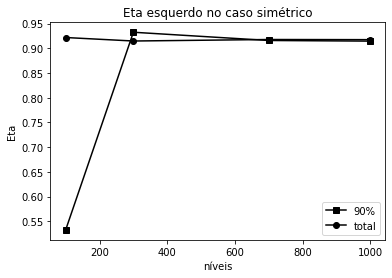
\includegraphics[width=\linewidth]{img/eta/eta_esquerdo_simetrico.png}
    	\end{subfigure}
    	\begin{subfigure}[b]{0.42\linewidth}
    		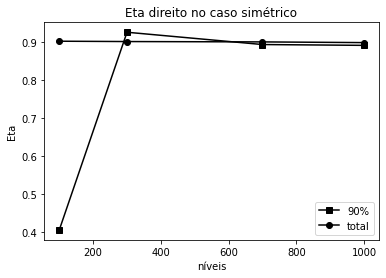
\includegraphics[width=\linewidth]{img/eta/eta_direito_simetrico.png}
    	\end{subfigure}
    	\caption{Valores de $\eta$ para as geometrias com o valor de \textit{standoff} 100\% ($A_1$ e $B_1$). Fonte: autor}
    	\label{fig:eta_simetrico}
    \end{figure}
    
    \begin{figure}[H]
        \centering
        \begin{subfigure}[b]{0.42\linewidth}
    		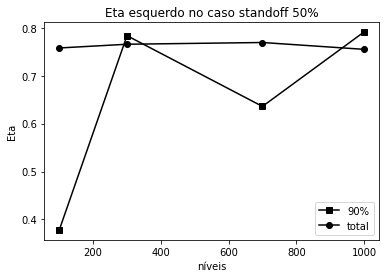
\includegraphics[width=\linewidth]{img/eta/eta_esquerdo_standoff.png}
    	\end{subfigure}
    	\begin{subfigure}[b]{0.42\linewidth}
    		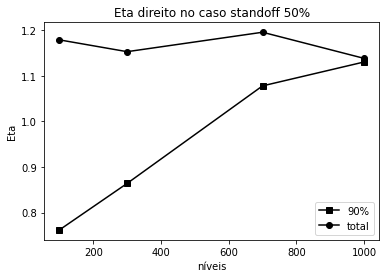
\includegraphics[width=\linewidth]{img/eta/eta_direito_standoff.png}
    	\end{subfigure}
    	\caption{Valores de $\eta$ para as geometrias com o valor de \textit{standoff} 50\%  ($A_2$ e $B_2$). Fonte: autor}
    	\label{fig:eta_standoff}
    \end{figure}
